\documentclass[10pt]{article}
\usepackage{multicol}
\usepackage{times}
\usepackage{graphicx}
\usepackage{mathtools}

\addtolength{\oddsidemargin}{-.875in}
\addtolength{\evensidemargin}{-.875in}
\addtolength{\textwidth}{1.75in}

\addtolength{\topmargin}{-.875in}
\addtolength{\textheight}{1.75in}


\begin{document}
\nocite{Gz:5}
\nocite{Gz:6}
\nocite{Gz:7}
\nocite{Gz:8}
\nocite{Gz:9}
\nocite{Gz:10}
\nocite{Gz:11}
\nocite{Gz:12}
\title{A Revised Implementation of the GRAPH/Z Graph Processing System}

\author{
  Ballmer, Alexander\\
  \texttt{alexandersballmer@gmail.com}
  \and
  Moudgalya, Shreyas\\
  \texttt{smoudgal@hawk.iit.edu}
}

\maketitle

\begin{abstract}
  The emerging applications in big data science and social networks has led to the development of several graph-parallel abstractions including GRAPH/Z. GRAPH/Z is a distributed parallel graph processing system running on top of ZHT, a zero hop distributed hash table. It uses an iterative vertex-centric model to store a large graph and run a variety of algorithms over it. GRAPH/Z has some performance issues, and cannot scale the same as Graphlab, a similar commercial framework. We hope to rewrite GRAPH/Z to be competitive with the commercial framework, Graphlab on a single node with multiple threads.  In the previous implementation GRAPH/Z used ZHT, a scalable distributed key-value store as building block. ZHT has very poor data locality, which can create performance issues. We also hope to develop a graph partitioning scheme that can be used in the loading process of GRAPH/Z.
\end{abstract}

\begin{multicols}{2} 
  \section{Background}
  GRAPH/Z was based off of a graph processing paradigm called Pregel. Pregel uses a model centered around the vertexes of the graph.\cite{Gz:1}  Each vertex has an update function that is run in the vertex's context in the graph. Vertexes can modify edges and send messages to other vertexes.\cite{Gz:1} The computation occurs in parallel iterations called supersteps.\cite{Gz:1} At each iteration, vertexes run an update function that can alter the edges around them, or send a message to vertexes in the next iteration. Vertexes can also vote to halt and disable themselves. A halted vertex can be re-enabled by receiving a message. If all the vertexes are disabled at the start of an iteration, the entire system halts and returns.\\
  GRAPH/Z adds a distributed hash table to the Pregel model. The hash table stores the graph, and a distributed message queue that serves as the means of sending messages to the next iteration. The hash table used by GRAPH/Z is ZHT, a DHT implementation that is fault-tolerant and can scale to 32000 cores.\cite{Gz:2}
  
  \section{Problem}
  \subsection{Scaling of GRAPHZ/Z}
  GRAPH/Z has experienced problems in terms of scaling competitively with commercial software like Graphlab because of the way that ZHT deals with data locality between nodes. ZHT's hashing function does not exploit data locality on one node.\cite{Gz:3} This can cause high network usage and slowdown.
  \section{Related Work}
  \subsection{Pregel}
  The closes related system to GRAPH/Z is Pregel. In most of our work, however, we compare GRAPH/Z to Graphlab, which is another high performance graph processing framework. Graphlab uses a similar paradigm to GRAPH/Z, but allows a vertex to access data that is not in a message to the vertex.\cite{Gz:4} \\
  Another less similar but still relevant work is Hadoop, which follows the MapReduce paradigm. GRAPH/Z and Pregel computations can be expressed as a series of chained MapReduce functions.\cite{Gz:4}
  
  \section{Proposed Solution}
  Our main work to solve our problems of scalability is to backtrack and try to achieve good scaling on a single node. We believe that the problem with GRAPH/Z lies in bad data locality with ZHT. Our main goal is to achieve some level of competitiveness against GraphLab on a single node, eventually expanding to multi-node scaling through ZHT or another distributed datastore. We will measure performance from weak scaling with larger datasets, and profiling tools such as valgrind/callgrind.
  
  \section{Evaluation}
  We will be using profiling tools such as valgrind and callgrind, along with basic runtime measurement, to measure the efficiency and speed of GRAPH/Z in relation to Graphlab. We will be using a modified pagerank algorithm defined as \\
  $\forall t \in P : r^{(t)}(t)  = (1-\alpha) \cdot r(t) + \alpha \sum_{(s,t) \in L} \frac{r^{(t-1)}(s)}{|L(s)|}$\\ 
  While profiling at a function call level will help us achieve our goal, the metrics used to determine success will be overall runtime and memory use. Scaling will be determined on multiple cores, and increasing data size, but on a single node.  These metrics will be used for the eventual later goal of scaling to more than one node.
\end{multicols}

  \section{Timeline}
  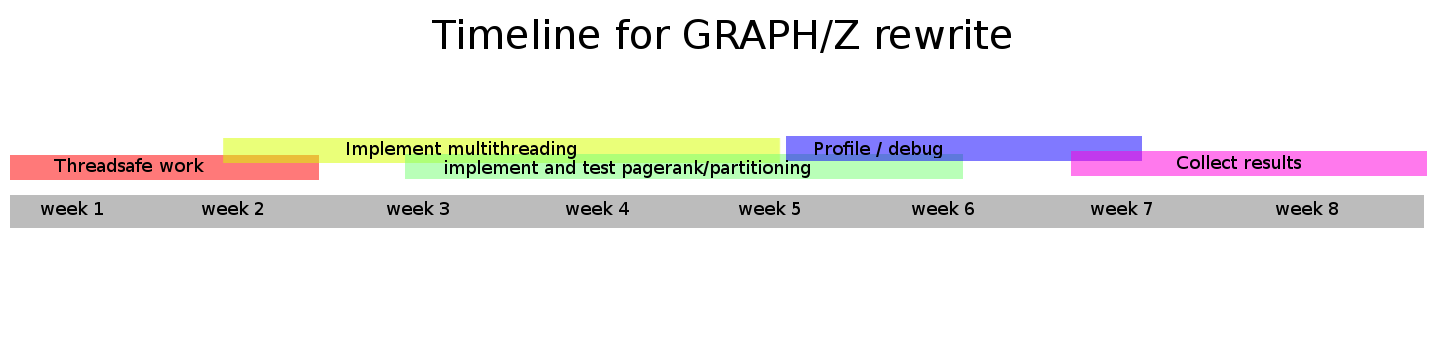
\includegraphics[width=\textwidth]{timeline.png}
\begin{multicols}{2}
  \section{Deliverables}
  We will produce a poster outlining the new GRAPH/Z's strengths and weaknesses and highlighting the changes that we made from the original project. The poster will also include the abstract and writeup needed for entering it into the Supercomputing conference.  Deliverables will also include the finished GRAPH/Z processing system and information comparing it to GraphLab and other existing similar tools. Included on the poster will be data from profiling and traces of the pagerank algorithm on a single local node  using the dataset from Stanford Network Analysis Project.
  
   \section{Conclusion}
   The original GRAPH/Z was underperforming compared to most other productions graph processing systems. We hope that rewriting it from scratch for a single node will help us pinpoint the cause of the lack of performance. In order to determine if the ZHT distributed hash table is an IO bottleneck, we will confine our implementation to a single node, and use an alternate backend besides ZHT. By using the newly proposed partitioning and pagerank algorithm on GRAPH/Z, we hope to measure better performance of the GRAPH/Z system.
   \bibliographystyle{plain}
   \bibliography{graphz}
\end{multicols}
\end{document}
